\chapter{Research Methodology}
\index{Research Methodology|(}

\noindent This chapter delineates the systematic approach employed to conduct the study, encompassing the research design, data collection methods, analysis procedures, and ethical considerations. Each section provides a comprehensive overview of the steps undertaken to ensure the research's validity and reliability.

\noindent This study will be divided into five (5) phases as shown in Table 3.1 below. The details of which are explained in sections 3.1 to 3.5, as follows.

\begin{table}[ht]
    \centering
    \renewcommand{\arraystretch}{1.5}
    \begin{tabular}{|c|p{4cm}|p{5cm}|p{4cm}|}
        \hline
        \textbf{Phase} & \textbf{Input} & \textbf{Process} & \textbf{Output} \\
        \hline
        1 & Institutional Documents (e.g., MSU-IIT Docs, BOR Resolutions), Sample Archives & Document collection and preparation (including scanned and text-based PDFs) & Curated Sample Document Set \\
        \hline
        2 & Literature Review, System Requirements & Design of system architecture integrating OCR (Marker), embedding (bge-m3), vector storage (pg\_vector), and interactive retrieval (Llama 3.2) & Detailed System Architecture \\
        \hline
        3 & System Architecture, Curated Sample Document Set & Implementation of core components: document ingestion, OCR processing, text chunking, batch embedding generation, vector storage, and chat interface & DRS Backend Prototype \\
        \hline
        4 & DRS Prototype, Sample Documents, Evaluation Metrics (e.g., SUS) & Performance evaluation of search accuracy, OCR quality, chunking coherence, vector retrieval relevance, and user experience & Evaluation Results \\
        \hline
        5 & Evaluation Results & Analysis of evaluation findings and documentation of feedback, improvements, and best practices & Final Documentation and Refined Framework \\
        \hline
    \end{tabular}
    \caption{\textit{Conceptual Framework of the Study}}
    \label{tab:conceptual-framework}
\end{table}
\index{Research Methodology|)}


\section{Process of Document Collection and Preparation}

\noindent The study begins with the collection and preparation of institutional documents, including MSU-IIT documents and BOR resolutions. Both scanned and text-based PDFs are gathered, curated, and pre-processed to serve as representative data for evaluating the new Document Retrieval System (DRS). This involves ensuring that a suitable range of document types, formats, and complexities (e.g., scanned documents requiring OCR) are included.

\section{Literature Review and System Architecture Design}

\noindent Informed by the collected data and user feedback, a comprehensive literature review is conducted to identify best practices and state-of-the-art techniques in content-based retrieval systems, OCR, vector embeddings, and large language model integration. This review guides the design of a system architecture that addresses identified shortcomings.

The proposed architecture integrates:

\begin{itemize}
    \item \textbf{OCR (Marker)}: Converting scanned PDFs into searchable text specifically converting it to markdown.
    \item \textbf{Dynamic Chunking}: Dividing markdown text into contextually coherent segments.
    \item \textbf{Embedding Generation (bge-m3)}: Transforming text segments into vector representations.
    \item \textbf{Vector Storage (pg\_vector on PostgreSQL)}: Efficient storage and similarity-based retrieval of embeddings.
    \item \textbf{Interactive Retrieval (Llama 3.2)}: Enabling users to engage in chat-based queries and receive contextually relevant responses.
\end{itemize}

\noindent A frontend developed in React ensures a user-friendly interface, while a Django-based backend and API layer handle data flow. Figure 3.1 illustrates the data pipeline from document ingestion to interactive retrieval, clarifying how each component fits into the overall architecture.

\begin{figure}[ht]
    \centering
    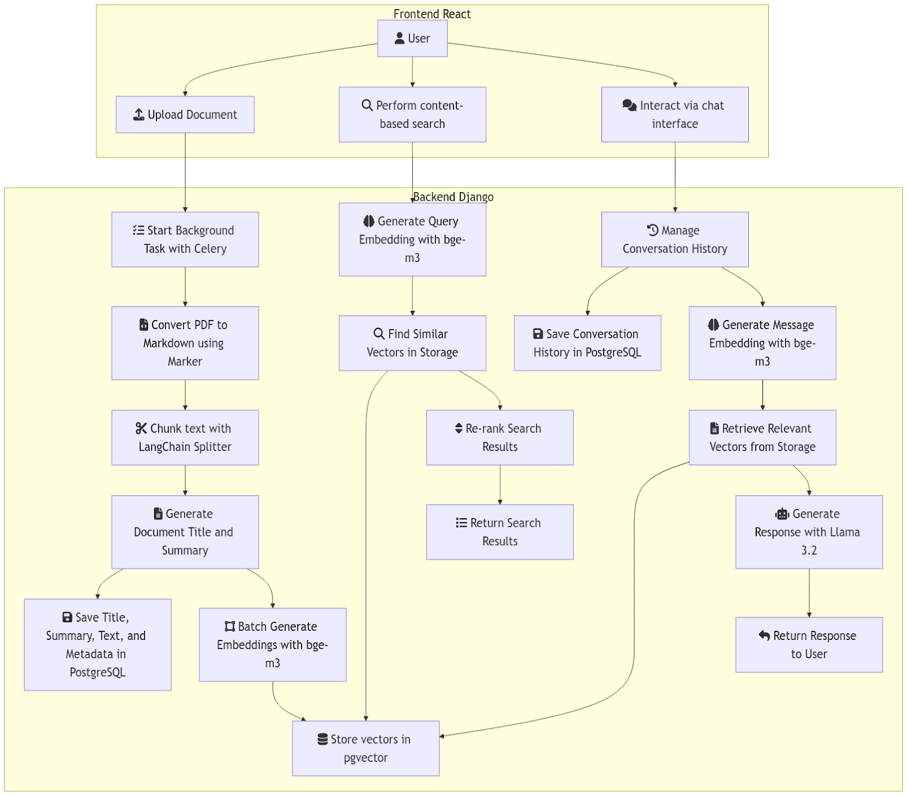
\includegraphics[width=0.9\textwidth]{thesis_architecture-design.png} % 
    \caption{\textit{System Workflow for Document Processing, Search, and Chat Interaction}}
    \label{fig:system-workflow}
\end{figure}

\section{Implementation of the Core Components}

\noindent With the architecture defined and a curated set of sample documents prepared, the DRS prototype is implemented. This phase focuses on integrating all core components into a unified system:

\begin{enumerate}
    \item \textbf{Document Ingestion \\& OCR}: When a user uploads a document, a background Celery task converts the file into Markdown (using Marker), ensuring that scanned PDFs become machine-readable.

    \item \textbf{Dynamic Chunking \\& Embedding}: Text is divided into context-rich chunks to maintain coherence. Batches of these chunks are embedded using the bge-m3 model, generating numerical vectors that represent semantic meaning.

    \item \textbf{Vector Storage \\& Retrieval}: The generated embeddings are stored in a PostgreSQL database enhanced with pg\_vector. This enables efficient similarity searches, ensuring that queries retrieve documents most relevant to the user’s needs.

    \item \textbf{Interactive Chat Interface}: On the frontend, users can perform content-based searches or engage in conversational queries. The backend processes user inputs, converts them into query embeddings, conducts a similarity search in the vector database, and uses Llama 3.2 to generate context-aware responses.
\end{enumerate}

\noindent System integration testing ensures the smooth operation of each component. Controlled scenarios are introduced to assess robustness, such as testing response quality under varying loads, handling corrupted file uploads, and simulating network interruptions.

\section{Performance Evaluation of the DRS Prototype}

\noindent To measure the system’s efficacy, approximately 50 test files with predetermined content are uploaded. Automated scripts simulate user actions—such as searching for specific terms, browsing results, and engaging in chat-based queries—to verify that the system returns accurate and context-relevant information.

\noindent Performance metrics include:

\begin{itemize}
    \item \textbf{Processing Accuracy}: Verifying that OCR and embedding pipelines produce correct outputs and that similarity searches yield semantically relevant documents.
    
    \item \textbf{Retrieval Efficiency}: Measuring query response times and system throughput under typical and peak usage conditions.
    
    \item \textbf{Robustness and Error Handling}: Introducing controlled faults (e.g., network interruptions, corrupted files) to confirm the system’s ability to recover gracefully without significant downtime or data loss.
\end{itemize}

\section{Analysis of Evaluation Results and Final Documentation}

\noindent After conducting performance evaluations, the results are analyzed and compared against the baseline established by the original keyword-based system. To ensure a direct and fair comparison of user satisfaction levels, the same survey instruments and respondent thresholds are applied to gather user feedback on the new content-based retrieval system. In usability testing, involving six participants per user group is often sufficient to uncover a significant portion of usability issues, balancing the need for actionable insights with resource constraints, as testing with more participants yields diminishing returns according to (\textit{A Guide to Usability Testing Sample Size - Trymata, 2024}).  Therefore, engaging six students, six faculty members, and six staff members in the evaluation process should provide a comprehensive understanding of the system's usability across different user groups.

\noindent The \textbf{System Usability Scale (SUS)} is employed to evaluate improvements in usability, satisfaction, and retrieval quality. SUS is a widely recognized and validated tool for assessing usability and provides a single score representing the overall user experience. This method is well-suited for capturing user perceptions through a standard 10-item questionnaire, generating results that are easy to interpret and benchmark. The combination of SUS scores and qualitative feedback ensures a comprehensive understanding of whether the new DRS meets or exceeds the functional and technical requirements derived from the initial studies.

\noindent The final step involves documenting the results, summarizing user feedback, detailing system improvements, and compiling best practices for future reference. The insights gained from the evaluation inform iterative refinements, ensuring the DRS evolves into a robust, user-centric solution that addresses the identified limitations of the previous retrieval system.
